% !TEX root = main.tex
\documentclass[a4paper, UKenglish, 11pt]{uiomaster}
\usepackage{lipsum}
\usepackage[subpreambles=true]{standalone}
\usepackage[table,xcdraw]{xcolor}
\usepackage{hyperref}
\usepackage{xcolor}

\begin{document}

\chapter{Extending the DiLoc Network}
In this chapter, we explore how various extensions and small modifications of the DiLoc network enhance its capability to address intricate and demanding inverse problems. We delve into three challenging scenarios, each designed to push the boundaries of DiLoc's predictive performance. The first extension involves assigning individual amplitudes to each dipole source, presenting the network with the task of predicting both the source locations and their corresponding amplitudes. Subsequently, the second scenario transitions from predicting the location of a single dipole source to estimating the center and radius of a population of dipoles, alongside the amplitude of the electrical signals generated. This extension introduces additional complexities to the localization process. Lastly, we investigate DiLoc's ability to predict the locations and amplitudes of two individual dipole sources that jointly contribute to the EEG signals recorded by the electrodes. These extensions aim to comprehensively evaluate the network's adaptability and generalization to increasingly intricate real-world situations. Throughout the chapter, we systematically evaluate the network's performance, providing insights into its strengths and limitations when confronted with these novel challenges.

\section{Predicting Single Dipole Sources with Amplitudes}

In this section, we introduce the concept of various amplitudes for single current dipole sources, which adds an additional dimension to the output of DiLoc. Besides predicting the coordinates of the dipoles for each sample, the network now also estimates the magnitude of the dipole signals. In real-world scenarios, it might be of interest to not only pinpoint the source of the abnormal activity but also comprehend the extent of abnormality. By incorporating amplitude prediction into our network, we gain valuable insights into the problem at hand and achieve a deeper understanding of the underlying brain activity.

% amplitude is too small ...  % include some sort of calculation of the stenght of the recording signal

\subsection{Adjustments in Data Set and Architecture}

We assign amplitudes to each dipole ranging between 1 and 10 nA$\mu$m. By now the dataset still has the same number of features, however the number of target values increases by 1. Figure \ref{fig:dipole_w_amplitude_example} provides two examples from the dataset, where the dipole location remains constant while the amplitude of the dipole signal varies. We observe that the shape of the EEG signal remain consistent, while the magnitude of the EEG signal is highest for the dipole with the largest amplitude. It should therefor not be a problem for the network to separate such cases and the network shold be able to provide accurate predictions for the amplitude in both cases. From the Figure it is also apperent that the EEG recordings ranges between -10 and 10 $\mu$V. \rednote{Can I find litterature that support the range?}

\begin{figure}[!htb]
    \centering
    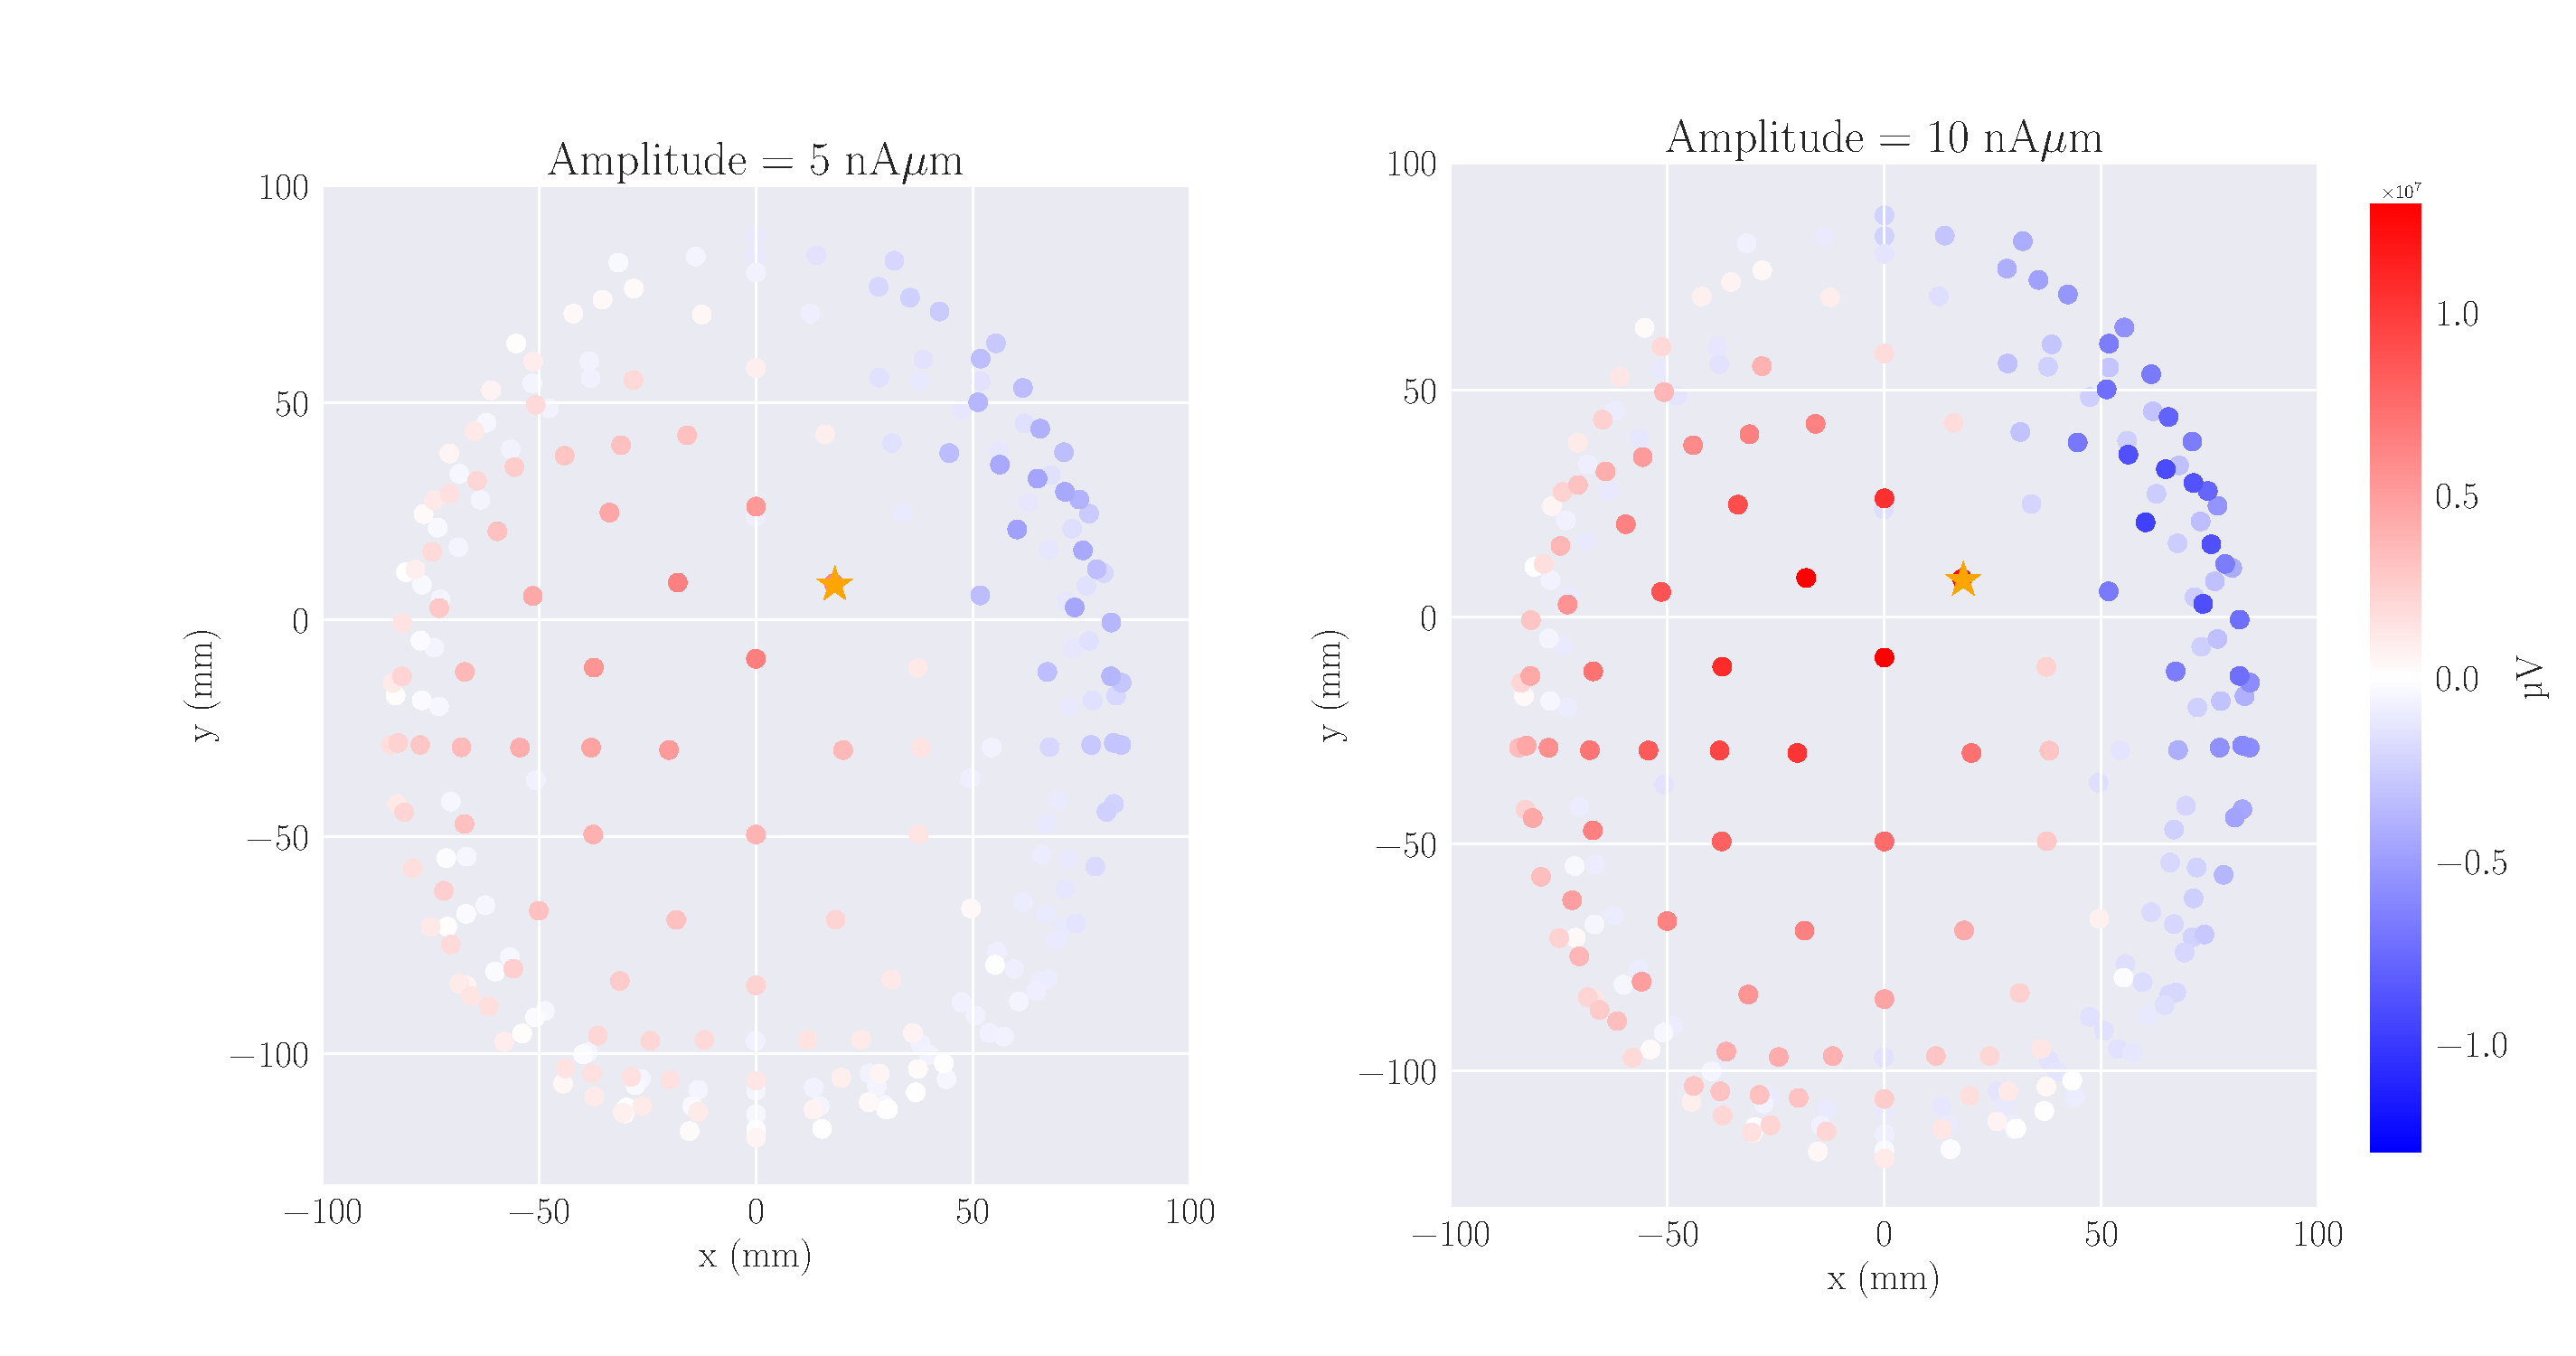
\includegraphics[width=\linewidth]{figures/dipole_w_amplitude_example.pdf}
    \caption{EEG data for two samples with current dipole amplitude equal to 5 and 10 nA$\mu$m. The EEG recordings have a range between -10 and 10 $\mu$V.}
    \label{fig:dipole_w_amplitude_example}
\end{figure}

In figure \ref{fig:NN_dipole_w_amplitude_architecture} we have depiced the construction of the extended DiLoc network, that now also provides for the amplitude. We see that DiLoc still takes an input of 231 data points corresponding to the number of recoring electrodes, however, the number of output nodes is increased by 1; x-coordinate, y-coordinate, z-coordinate and amplitude corresponding to the strenght of the signal for the current dipole moment in the cortex.

\begin{figure}[!htb]
    \centering
    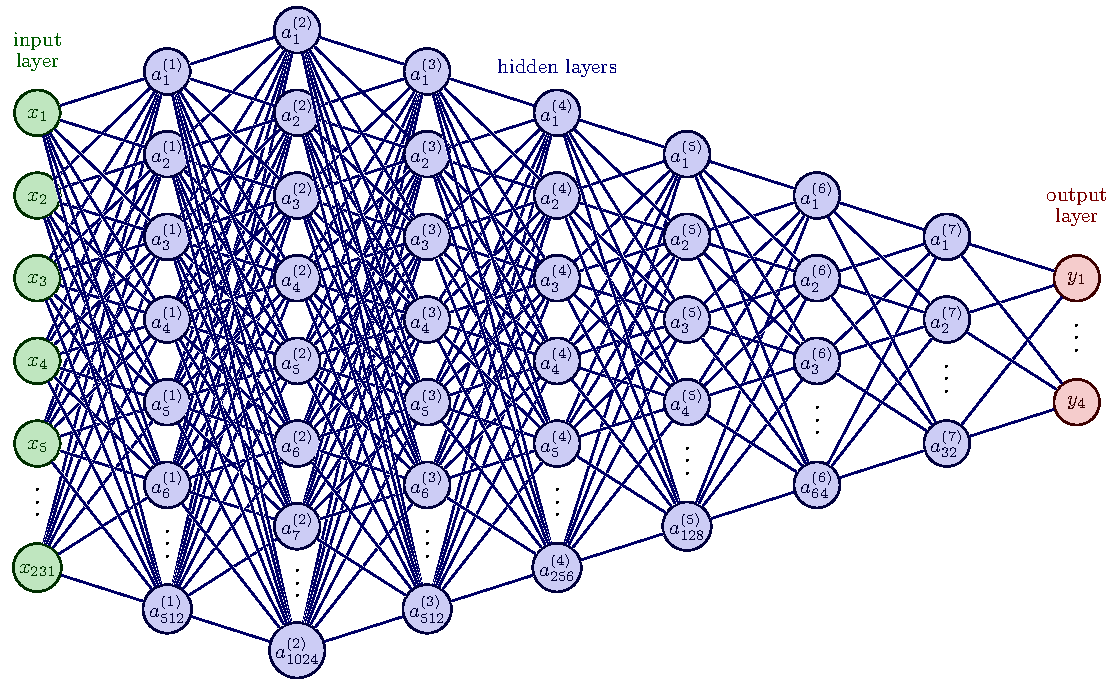
\includegraphics[width=\linewidth]{figures/NN_dipole_w_amplitude_architecture.pdf}
    \caption{Architecture dipole with amplitude.}
    \label{fig:NN_dipole_w_amplitude_architecture}
\end{figure}

As was done for the previous problem, the input data is scaled by subtracting the mean and dividing on the variance. However, as DiLoc deals with multipole output units, specifically millimeters (mm) and nanoampere-micrometers (nA$\mu$m), a scaling process is implemented also on the output targets to effectively minimize the cost function. The cost function calculates the differences between the predicted output and the actual target values. When output values have different ranges and units, there is a risk that certain dimensions of the target values may dominate the overall error calculation, while others with smaller ranges might be neglected. Consequently, the neural network might overly prioritize reducing errors in the larger range values, hindering its ability to accurately learn patterns and generalize well for the smaller range values.

To address this issue, the output values are normalized to a common range of 0 to 1 using the following normalization formula:

\begin{equation}
z_i = \frac{x_i - \text{min}(x)}{\text{max}(x) - \text{min}(x)}
\label{eq:scale_target}
\end{equation}

Here, $z_i$ represents the i$^{\text{th}}$ normalized value in the dataset for a specific target category, $x_i$ is the i$^{\text{th}}$ value in the corresponding target dataset, and min($x$) and max($x$) are the minimum and maximum values in that specific target dataset.

It is important to perform this normalization separately for each target category. Doing so allows the neural network to effectively train and discern patterns using only one cost function. Without this normalization, employing a single cost function for a set of different target values with distinct units would not be feasible. By applying this normalization, we aim to provide a more balanced cost function where all target values contribute equally to the overall error calculation. Consequently, the network can learn effectively from the data and achieve better results in its tasks.

% Is it true that sigmoid helpt the efficentcy of the lerning process for the network? For improvements, it would be beneficial to elaborate on the rationale behind using hyperbolic tangent for the hidden layers and ReLU for the first layer.
In the extension of the DiLoc network, we maintain the use of ReLU as the activation function in the first layer, and hyperbolic tangent for the hidden layers, as this architecture, combined with the choise of parameter valued gave the best results. However, considering that the output data has been normalized to a range from 0 to 1, we deem it appropriate to employ the Sigmoid activation function in the output layer. The Sigmoid function maps the output values to a range between 0 and 1, which aligns with our desired output range. This choice may potentially facilitate the training process, as it enables the network to converge more effectively towards the desired outputs. %Nonetheless, it is important to emphasize that the efficacy of this activation function in improving the learning process should be further validated through empirical experiments or referenced studies.

As for the simple DiLoc model, we continue to utilize the technique of adaptive learning rate, which can be advantageous for optimizing the network's parameters more efficiently. For an overview of the overall parameters employed in the model, please refer to Table \ref{table:parameters}, which provides a summary of these essential elements.

\begin{table}[]
\begin{tabular}{|lc|}
\hline
\rowcolor[HTML]{CBCEFB}
\multicolumn{2}{|c|}{\cellcolor[HTML]{CBCEFB}{\color[HTML]{000000} \textbf{DiLoc for localizing current dipoles with amplitude}}}    \\ \hline
\rowcolor[HTML]{EFEFEF}
\multicolumn{1}{|l|}{\cellcolor[HTML]{EFEFEF}\textbf{Hyperparameters}} & \multicolumn{1}{l|}{\cellcolor[HTML]{EFEFEF}\textbf{Value}} \\ \hline
\multicolumn{1}{|l|}{Hidden layers}                                    & 6                                                           \\ \hline
\multicolumn{1}{|l|}{Optimizer}                                        & SGD                                                         \\ \hline
\multicolumn{1}{|l|}{Learning rate (initial)}                          & 0.001                                                       \\ \hline
\multicolumn{1}{|l|}{Momentum}                                         & 0.35                                                        \\ \hline
\multicolumn{1}{|l|}{Weight decay}                                     & 0.1                                                         \\ \hline
\multicolumn{1}{|l|}{Minibatch size}                                   & 32                                                          \\ \hline
\multicolumn{1}{|l|}{Epochs}                                           & 5000                                                        \\ \hline
\multicolumn{1}{|l|}{Dropout}                                          & 0.5                                                         \\ \hline
\multicolumn{1}{|l|}{Act.func in first layer}                                          & ReLU                                                         \\ \hline
\multicolumn{1}{|l|}{Act.func in hidden layers}                                          & Tanh                                                         \\ \hline
\multicolumn{1}{|l|}{Act.func in last layer}                                          & Sigmoid                                                         \\ \hline
\end{tabular}
\label{tab:parameters}
\end{table}

\subsection{Performance Evaluation}

To assess the network's performance, we start by analyzing the accuracy in relation to training epochs, as depicted in Figure \ref{fig:dipole_w_amplitude_loss}. It is important to note that the target values have been normalized, resulting in a unitless loss measurement. Therefore, the figure provides a qualitative representation of the network's training progress rather than precise loss values. The plot clearly demonstrates a consistent pattern of decreasing loss as the number of epochs increases, indicating that the network effectively captures the underlying data patterns. Moreover, both the training and validation loss stabilize after approximately 2000 epochs, suggesting that the network may have reached its optimal performance level. In Figure \ref{fig:dipole_w_amplitude_targets}, we present the loss development for different target values. Once again, we observe that the loss stabilizes at around 2000 epochs. Notably, for the x-, z-, and y-coordinates, the stabilized loss corresponds to the minimum value reached during the training period. However, for the amplitude target value, this is not the case. From the provided figure, it is apparent that the smallest loss value occurs in a sharp dip just before reaching 500 epochs. This observation implies that if we solely aimed to minimize the loss function with respect to the amplitude value, the most optimal model would have emerged by terminating the training process at that epoch. However, since our objective is to develop a model that accurately predicts both the location and amplitude of the current dipole, we strive to train the model until the total loss is minimized, encompassing both aspects.

\begin{figure}[!htb]
    \centering
    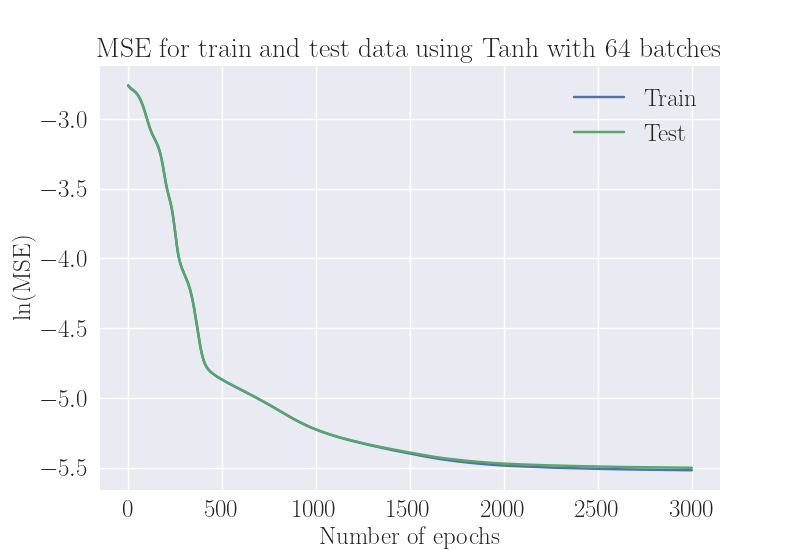
\includegraphics[width=\linewidth]{figures/MSE_tanh_50000_3july_mseloss_MSE_dipole_w_amplitude_3000_SGD_lr0.001_wd0.1_mom0.35_bs64_Tanh_64_3000_N_dipoles_1.png}
    \caption{The loss for the extended DiLoc network with 50 000 samples and hyperbolic tangent activation function.}
    \label{fig:dipole_w_amplitude_loss}
\end{figure}

\begin{figure}[!htb]
    \centering
    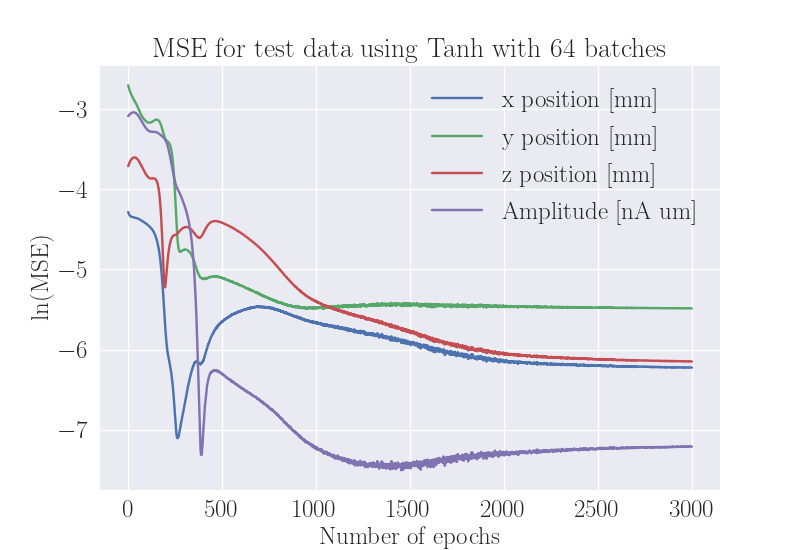
\includegraphics[width=\linewidth]{figures/mse_targets_tanh_50000_3july_mseloss_MSE_dipole_w_amplitude_3000_SGD_lr0.001_wd0.1_mom0.35_bs64.png}
    \caption{The loss developmnent for the different target values as function of epochs.}
    \label{fig:dipole_w_amplitude_targets}
\end{figure}

In Table \ref{table:error_simple_dipole} we have provided the performance of the network by concidering different error metrics. The mean absolute error (MAE) values for the x-, y-, and z- coordinates rnage from 0.8300 mm to 0.8998 mm. This means that, on average, the network's predictions have an error smaller than 1 mm in each coordinate. Considering the range of the coordinates, the MAE values represent a reasonable level of accuracy. The mean squared error penalizes larger errors/outliers more severely than MAE since it involves squaring the differences. In our case the MSE values for the different coordinates range from 1.2134 mm to 1.4110 mm. The hugher MSE values suggest that the predictions of the network may have larger errors in some cases, resulting in a higher average squared difference. However, the magnitude of the mean squared errors is still whithin a reasonable range when analyzing them in the context of the coordinates ranges. Finally the root mean squared error provides a measure of the standard deviation of the errors and helps to understand the spread of errors around the mean. The RMSE values of ours are slighly lower than the corresponding MSE values with a range from 1.1016 mm to 1.1878 mm. The table also presents the error metrics calculated for the euclidean distance. For both MAE, MSE and RMSE the value is higher than the individual coordinate errors, indicating that the errors in the x, y, and z coordinates are not perfectly aligned and contribute to the overall distance. It is worth mentioning that specific points in the cortex matrix may potentially contribute more to the errors. Further investigation could be performed to identify any specific patterns or regions in the cortex that exhibit higher error rates. However, overall the results indicate that the network is able to predict the dipole location with reasonable accuracy. While there are some errors in the predictions, the errors are generally within an acceptable range.

% Please add the following required packages to your document preamble:
% \usepackage[table,xcdraw]{xcolor}
% If you use beamer only pass "xcolor=table" option, i.e. \documentclass[xcolor=table]{beamer}
\begin{table}[!htb]
\begin{tabular}{l|
>{\columncolor[HTML]{FFFFFF}}c
>{\columncolor[HTML]{FFFFFF}}c
>{\columncolor[HTML]{FFFFFF}}c
>{\columncolor[HTML]{FFFFFF}}c
>{\columncolor[HTML]{FFFFFF}}c |}
\cline{2-6}
                                                   & \multicolumn{5}{c|}{\cellcolor[HTML]{CBCEFB}\textbf{Error for different target values}}                                                                                                                                                                                                                                                                                                                                                                                                                                                                                            \\ \cline{2-6}
                                                   & \multicolumn{1}{l|}{\cellcolor[HTML]{EFEFEF}\begin{tabular}[c]{@{}l@{}}x-coordinate\\ {[}mm{]}\end{tabular}} & \multicolumn{1}{l|}{\cellcolor[HTML]{EFEFEF}\begin{tabular}[c]{@{}l@{}}y-coordinate\\ {[}mm{]}\end{tabular}} & \multicolumn{1}{l|}{\cellcolor[HTML]{EFEFEF}\begin{tabular}[c]{@{}l@{}}z-coordinate\\ {[}mm{]}\end{tabular}} & \multicolumn{1}{l|}{\cellcolor[HTML]{EFEFEF}\begin{tabular}[c]{@{}l@{}}Euclidean \\ Distance {[}mm{]}\end{tabular}} & \multicolumn{1}{l|}{\cellcolor[HTML]{EFEFEF}\begin{tabular}[c]{@{}l@{}}Amplitude\\ {[}nA$\mu$m{]}\end{tabular}} \\ \hline
\multicolumn{1}{|l|}{\cellcolor[HTML]{EFEFEF}MAE}  & \multicolumn{1}{c|}{\cellcolor[HTML]{FFFFFF}3.627}                                                           & \multicolumn{1}{c|}{\cellcolor[HTML]{FFFFFF}4.006}                                                           & \multicolumn{1}{c|}{\cellcolor[HTML]{FFFFFF}3.476}                                                           & \multicolumn{1}{c|}{\cellcolor[HTML]{FFFFFF}2.949}                                                                  & 0.687                                                                                                           \\ \hline
\multicolumn{1}{|l|}{\cellcolor[HTML]{EFEFEF}MSE}  & \multicolumn{1}{c|}{\cellcolor[HTML]{FFFFFF}22.595}                                                          & \multicolumn{1}{c|}{\cellcolor[HTML]{FFFFFF}28.128}                                                          & \multicolumn{1}{c|}{\cellcolor[HTML]{FFFFFF}22.006}                                                          & \multicolumn{1}{c|}{\cellcolor[HTML]{FFFFFF}18.410}                                                                 & 0.687                                                                                                           \\ \hline
\multicolumn{1}{|l|}{\cellcolor[HTML]{EFEFEF}RMSE} & \multicolumn{1}{c|}{\cellcolor[HTML]{FFFFFF}4.753}                                                           & \multicolumn{1}{c|}{\cellcolor[HTML]{FFFFFF}5.306}                                                           & \multicolumn{1}{c|}{\cellcolor[HTML]{FFFFFF}4.691}                                                           & \multicolumn{1}{c|}{\cellcolor[HTML]{FFFFFF}4.291}                                                                  & 0.938                                                                                                           \\ \hline
\end{tabular}
\caption{\textbf{Evaluation of the network performance utializing different Error Metrics.} \newline
Performance for the extended DiLoc network on test dataset consisting of 1000 samples. The errors are measured using Mean Squared Error (MSE), Mean Absolute Error (MAE), and Root Mean Squared Error (RMSE).}
\label{table:error_simple_dipole}
\end{table}



\section{Predicting Region of Active Correlated Current Dipoles with Amplitudes}

In order to further enhance the complexity of our problem, we extend the DiLoc neural network to incorporate varying radii and amplitudes for the origins generating the electrical activity detected by the recording electrodes. This transformation alters the objective of the DiLoc network from predicting the location of individual current dipole moments to estimating the centers of larger spherical populations. This extension is valuable for real-life scenarios where understanding the extent of brain damage causing abnormal activity in damaged areas may be of interest. By training the DiLoc network on such complex data, we aim to enhance its ability to generalize and perform effectively in real-world clinical cases.

\subsection{Adjustments in Data Set and Architecture}
% Include that with this arcitecture the amplitude/radius is more weighted than position (maybe)...

For the purpose of enabling the network to predict the areas of dipole populations, we make adjustments to the dataset. The dipole populations are represented as spherical volumes in the NY head cortex, with the radius for each population ranging from 1 mm to 15 mm. To ensure realism, we maintain the maximum amplitude strength of the total populations at 10 mA$\mu$m. Consequently, we calculate the maximum number of points within a volume sphere with a radius of 15 mm and reduce this number by 10 to determine the strength of each dipole within the given area. This leaves us with a strength of 10/899 for each dipole. The strength of a dipole population is thus directly proportional to the size of the dipole population. While this may not perfectly represent real-world scenarios, it provides a reasonable approximation for our model.

In Figure \ref{fig:dipole_area}, we present an example of a dipole population and the corresponding EEG signal. The yellow filled circles in the plots in the upper panel represents the diple populations, i.e. positions within the cortex where dipoles have been placed. The lower panel shows the EEG signals for the specific sample, with EEG electrode locations presented as filled circles, where the color of the fill represents the amplitude of the measured signal for the given electrode. The plots within the figure are seen from both the x-z plane, x-y plane, and the y-z plane.

\begin{figure}[!htb]
\centering
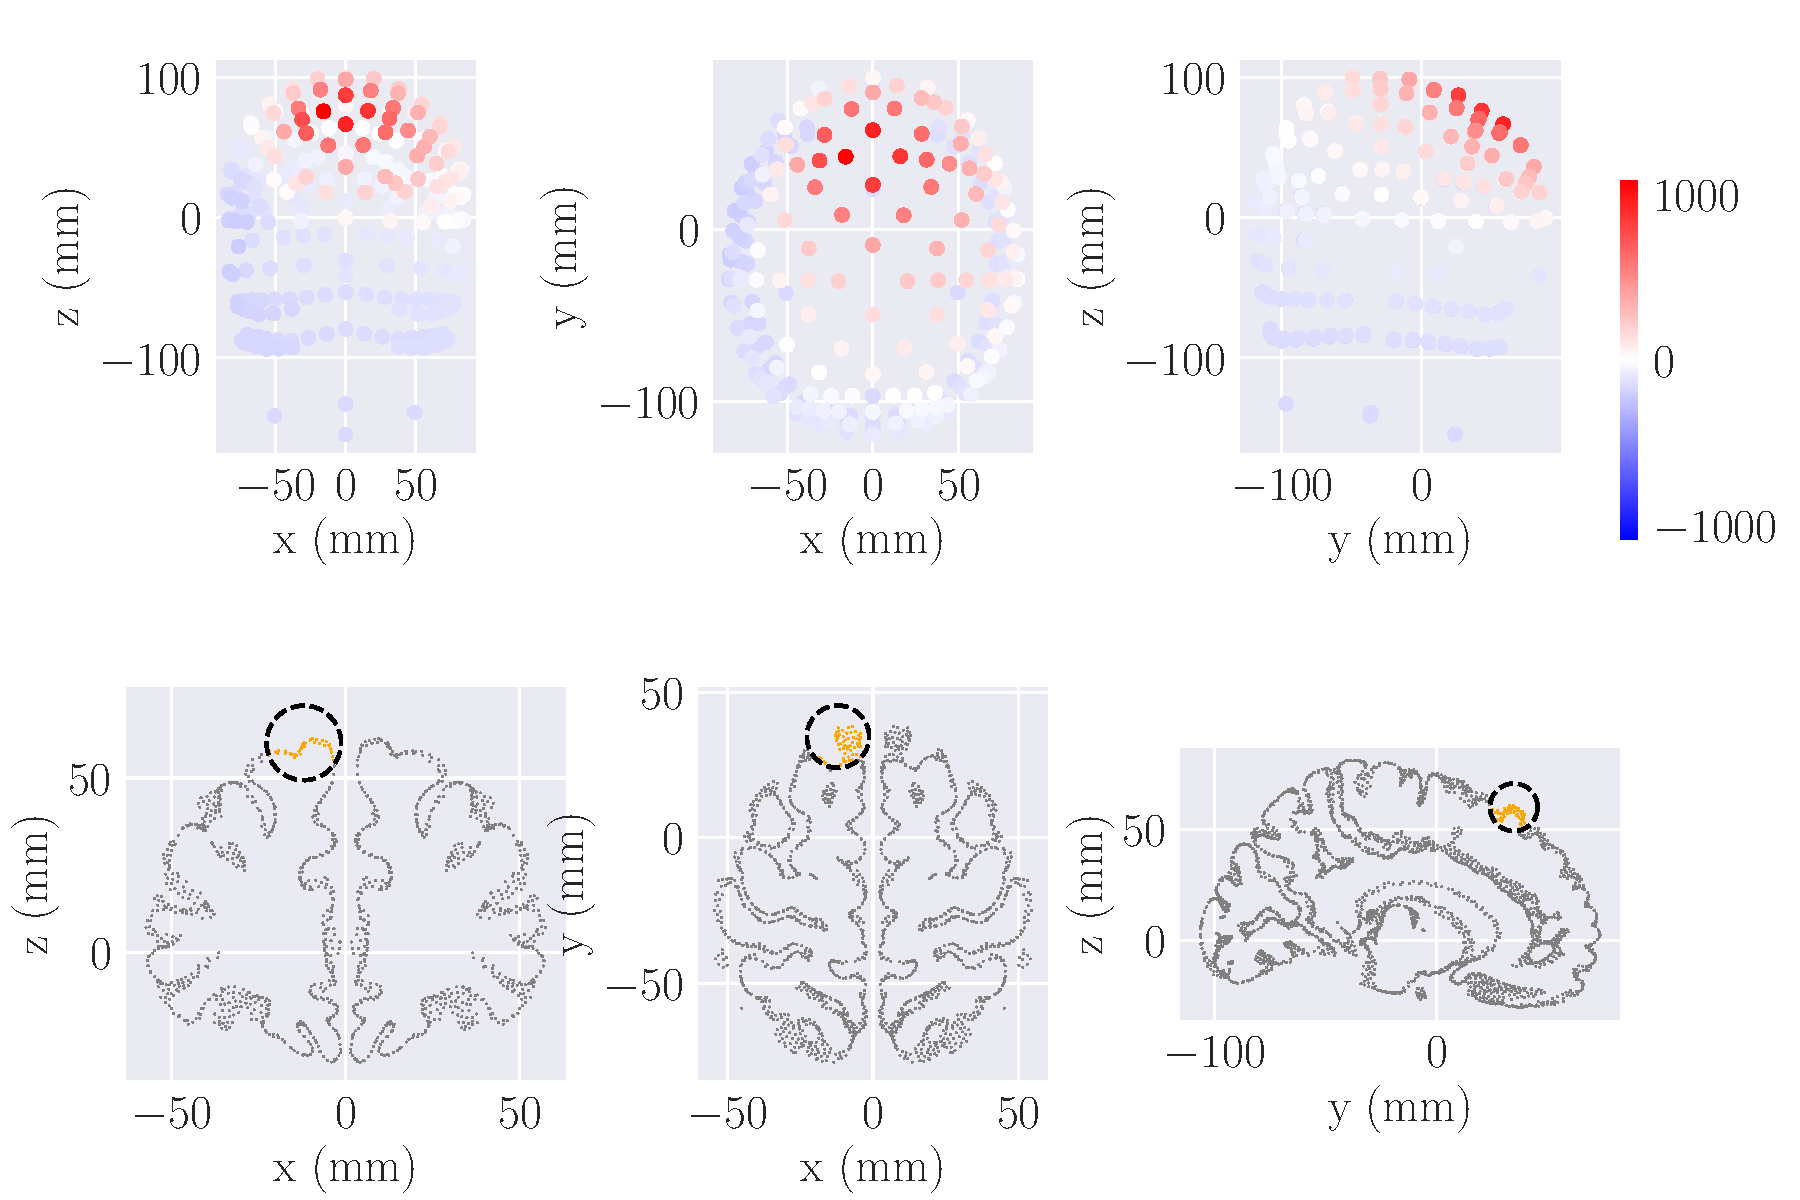
\includegraphics[width=\linewidth]{figures/dipole_area_reduced_0.pdf}
\caption{EEG for a sample containing a spherical population of current dipole sources with a random center within the cerebral cortex. The EEG measure is seen from both sides (x-z plane and y-z plane) and above (the x-y plane). EEG electrode locations are presented as filled circles, where the color of the fill represents the amplitude of the measured signal for the given electrode.}
\label{fig:dipole_area}
\end{figure}

As for the dataset, the number of target values is now 5: x, y, z-coordinates of the center of the dipole population, amplitude, and radius. The number of features is not modified and still holds the number of 231, representing the recording electrodes. The new architecture of the DiLoc network is presented in Figure \ref{fig:NN_dipole_area_architecture.pdf}.

\begin{figure}[!htb]
\centering
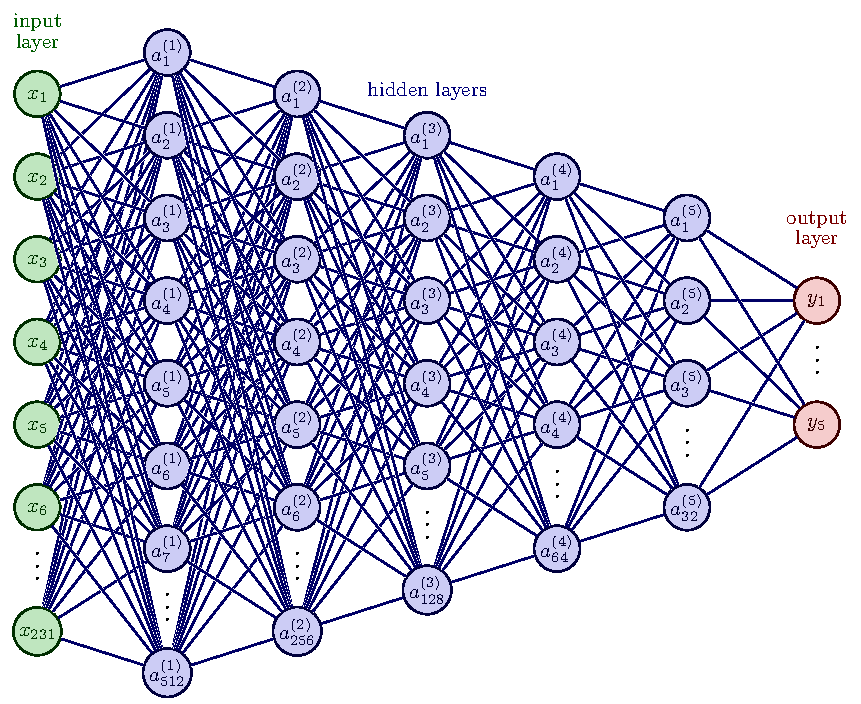
\includegraphics[width=\linewidth]{figures/NN_dipole_area_architecture.pdf}
\caption{Architecture of the dipole area prediction network.}
\label{fig:NN_dipole_area_architecture}
\end{figure}

Similar to the previous problem, we normalize the target values to ensure they all range from 0 to 1. Moreover, in this extension of the DiLoc network, we use the same activation functions as in the previous problem with ReLU as the activation function in the first layer, hyperbolic tangent for the hidden layers, and the Sigmoid activation function in the output layer. As with the previous problems, we have explored various network architectures and activation functions, but the current configuration has shown the best performance in terms of accurate predictions for this problem. It is important to emphasize that our primary goal is to find a network that can effectively solve the problem and provide accurate predictions, rather than necessarily seeking the best possible configuration.


\subsection{Performance Evaluation}
% How does the loss relate to size of population
% Exammple run and how long time it takes to calculate

In Figure \ref{fig:dipoile_area_result}, we present the training and validation Mean Squared Error (MSE) loss for the ConvDip network as a function of epochs. The network was trained for 5000 epochs, but the validation loss appears to converge at around 3000 epochs, while the training loss stabilizes at approximately 4000 epochs. Notably, there are no signs of overfitting, which is a positive outcome. Each epoch took approximately 7 seconds, resulting in a total training period of approximately 9 hours.

Figure \ref{fig:dipole_area_target_result} displays the validation loss for each target value as a function of epochs. The losses for all coordinate target values (x, y, and z) are minimized almost identically, with the y-coordinate loss slightly smaller. The amplitude target value is minimized most effectively by ConvDip, while the radius target value has the highest loss. We keep in mind that the amplitude and radius taget value correlates to some extent, as the amplitude is proportional to the radius. Although the exact MSE values for the target values cannot be directly read from the figure due to normalization, the overall pattern indicates that ConvDip successfully captures data patterns and minimizes the cost function.


\begin{figure}[!htb]
    \centering
    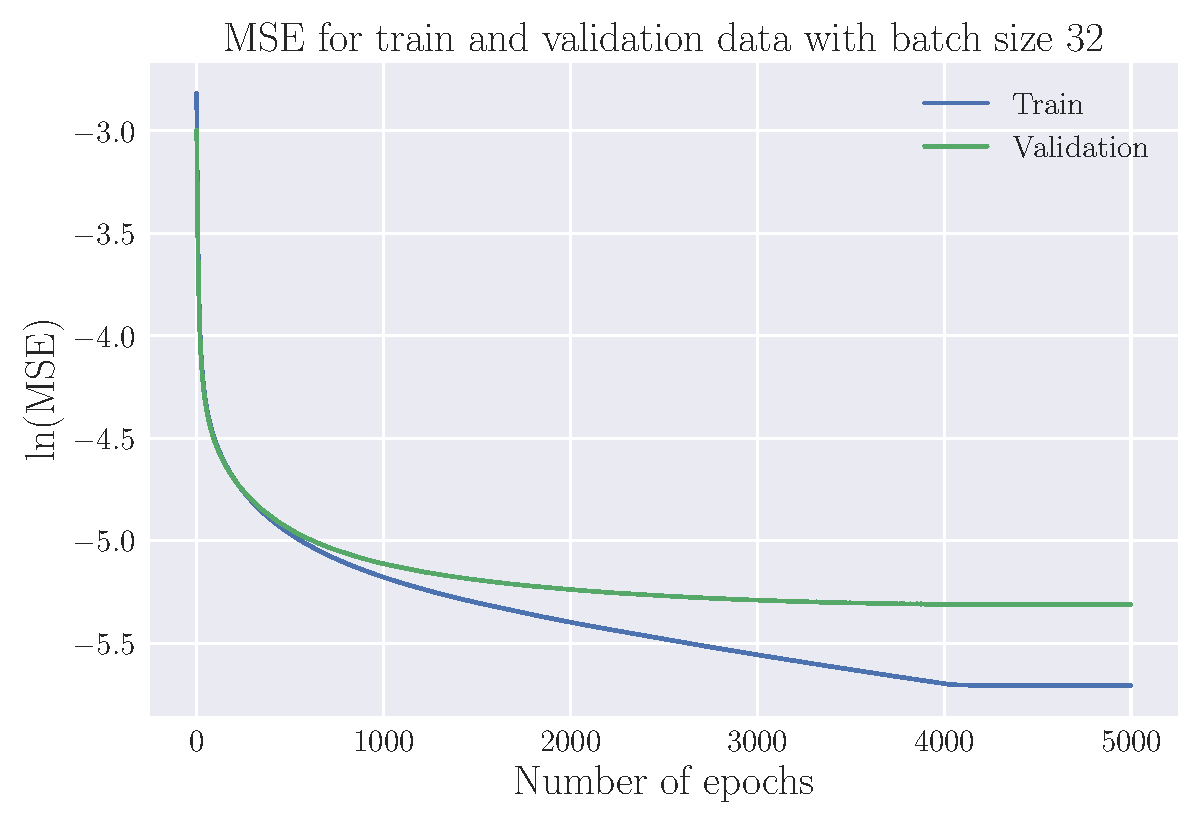
\includegraphics[width=\linewidth]{figures/mse_area_32_0.001_0.35_0.1_0.0_5000_(0).pdf}
    \caption{The validation accuracy for the simple Feed Forward Neural Network, predicting both center and radius for 50 000 samples, for 5000 epochs, with a learning rate equal to 0.001.}
    \label{fig:dipole_area_result}
\end{figure}

\begin{figure}[!htb]
    \centering
    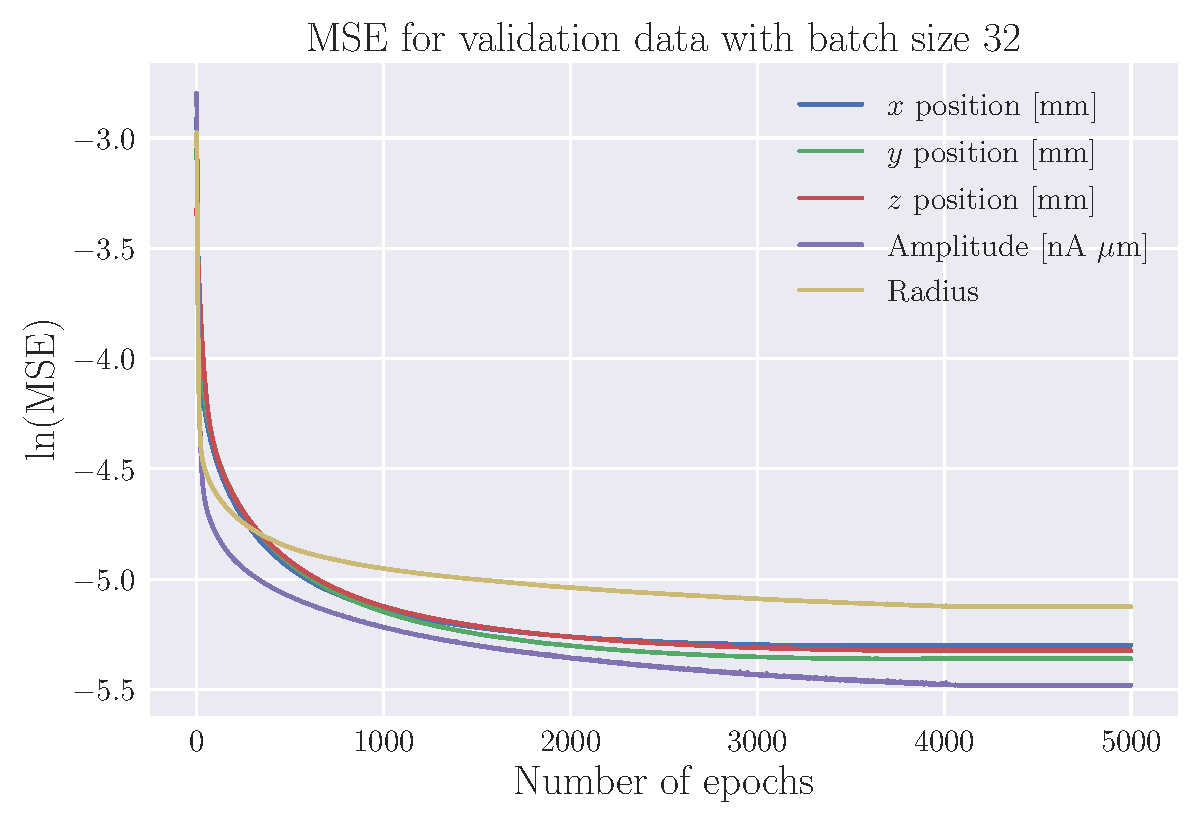
\includegraphics[width=\linewidth]{figures/mse_targets_area_32_0.001_0.35_0.1_0.0_5000_(0).pdf}
    \caption{The validation accuracy as function of epoch for each target value: x, y, z-coordinates of the center of the dipole population, amplitude, and radius. }
    \label{fig:dipole_area_target_result}
\end{figure}


To assess the extent to which the network can predict the center of the dipole populations, in addition to amplitude and radius, we utilize the same evaluation metrics as described in chapter 6. Table \ref{table:error_dipole_area} presents the Mean Absolute Error (MAE), Normalized MEan Absolute Error (NMAE), Mean Squared Error (MSE), and Root Mean Squared Error (RMSE) for the different sets of target parameters.

The MAEs for all coordinates and the Euclidean distance lie between 4 and 5 millimeters. Looking at the NMAE, we observe that the loss for the z-coordinate is somewhat larger than for the other coordinates, with 3 $\%$, similar to our observations when testing DiLoc's ability to predict amplitude in addition to location. However, this slightly larger error is not significant and may as well be attributed to randomness. What is worth mentioning is that all cordinates


As for the amplitude and radius targets, the MAEs are remarkably small. For amplitude, ranging from 1 to 10 mA$\mu$m, the absolute error is approximately 4.33$\%$ of the range of the actual amplitude values, indicating that the model's amplitude predictions are reasonably close to the true amplitude values. Similarly, the MAE for the radius, with a range from 1 to 15 mm, is approximately 6.07$\%$, suggesting that the model's predictions are relatively accurate for radius.

Regarding the MSE, we observe relatively small errors for the amplitude and radius, with values of 0.364 and 1.291 (mm$^2$) respectively. However, as for the coordinate target values, we encounter relatively larger MSE values. This difference in scale between the MAE and MSE suggests the presence of outliers.





    % Please add the following required packages to your document preamble:
    % \usepackage[table,xcdraw]{xcolor}
    % If you use beamer only pass "xcolor=table" option, i.e. \documentclass[xcolor=table]{beamer}
    \begin{table}[]
    \begin{tabular}{c|
    >{\columncolor[HTML]{FFFFFF}}c
    >{\columncolor[HTML]{FFFFFF}}c
    >{\columncolor[HTML]{FFFFFF}}c
    >{\columncolor[HTML]{FFFFFF}}c
    >{\columncolor[HTML]{FFFFFF}}c
    >{\columncolor[HTML]{FFFFFF}}c |}
    \cline{2-7}
    \multicolumn{1}{l|}{}                              & \multicolumn{6}{c|}{\cellcolor[HTML]{CBCEFB}\textbf{Error for different target values}}                                                                                                                                                                                                                                                                                                                                                                                                                                                                                                                                                             \\ \cline{2-7}
    \multicolumn{1}{l|}{}                              & \multicolumn{1}{c|}{\cellcolor[HTML]{EFEFEF}\begin{tabular}[c]{@{}c@{}}x \\ {[}mm{]}\end{tabular}} & \multicolumn{1}{c|}{\cellcolor[HTML]{EFEFEF}\begin{tabular}[c]{@{}c@{}}y \\ {[}mm{]}\end{tabular}} & \multicolumn{1}{c|}{\cellcolor[HTML]{EFEFEF}\begin{tabular}[c]{@{}c@{}}z \\ {[}mm{]}\end{tabular}} & \multicolumn{1}{l|}{\cellcolor[HTML]{EFEFEF}\begin{tabular}[c]{@{}l@{}}Center \\ {[}mm{]}\end{tabular}} & \multicolumn{1}{l|}{\cellcolor[HTML]{EFEFEF}\begin{tabular}[c]{@{}l@{}}Amplitude \\ {[}nA$\mu$m{]}\end{tabular}} & \multicolumn{1}{l|}{\cellcolor[HTML]{EFEFEF}\begin{tabular}[c]{@{}l@{}}Radius \\ {[}mm{]}\end{tabular}} \\ \hline
    \multicolumn{1}{|c|}{\cellcolor[HTML]{EFEFEF}MAE}  & \multicolumn{1}{c|}{\cellcolor[HTML]{FFFFFF}4.257}                                                 & \multicolumn{1}{c|}{\cellcolor[HTML]{FFFFFF}4.868}                                                 & \multicolumn{1}{c|}{\cellcolor[HTML]{FFFFFF}4.126}                                                 & \multicolumn{1}{c|}{\cellcolor[HTML]{FFFFFF}4.417}                                                      & \multicolumn{1}{c|}{\cellcolor[HTML]{FFFFFF}0.390}                                                               & 0.850                                                                                                   \\ \hline
    \multicolumn{1}{|c|}{\cellcolor[HTML]{EFEFEF}NMAE} & \multicolumn{1}{c|}{\cellcolor[HTML]{FFFFFF}2.955}                                                 & \multicolumn{1}{c|}{\cellcolor[HTML]{FFFFFF}2.711}                                                 & \multicolumn{1}{c|}{\cellcolor[HTML]{FFFFFF}3.083}                                                 & \multicolumn{1}{c|}{\cellcolor[HTML]{FFFFFF}2.916}                                                      & \multicolumn{1}{c|}{\cellcolor[HTML]{FFFFFF}4.333}                                                               & 6.071                                                                                                   \\ \hline
    \multicolumn{1}{|c|}{\cellcolor[HTML]{EFEFEF}MSE}  & \multicolumn{1}{c|}{\cellcolor[HTML]{FFFFFF}47.141}                                                & \multicolumn{1}{c|}{\cellcolor[HTML]{FFFFFF}68.776}                                                & \multicolumn{1}{c|}{\cellcolor[HTML]{FFFFFF}46.192}                                                & \multicolumn{1}{c|}{\cellcolor[HTML]{FFFFFF}54.036}                                                     & \multicolumn{1}{c|}{\cellcolor[HTML]{FFFFFF}0.364}                                                               & 1.291                                                                                                   \\ \hline
    \multicolumn{1}{|c|}{\cellcolor[HTML]{EFEFEF}RMSE} & \multicolumn{1}{c|}{\cellcolor[HTML]{FFFFFF}6.866}                                                 & \multicolumn{1}{c|}{\cellcolor[HTML]{FFFFFF}8.293}                                                 & \multicolumn{1}{c|}{\cellcolor[HTML]{FFFFFF}6.796}                                                 & \multicolumn{1}{c|}{\cellcolor[HTML]{FFFFFF}7.351}                                                      & \multicolumn{1}{c|}{\cellcolor[HTML]{FFFFFF}0.604}                                                               & 1.136                                                                                                   \\ \hline
    \end{tabular}
    \caption{\textbf{Evaluation of DiLoc utilizing different Error Metrics.}
    Performance of the extended DiLoc network on a test dataset consisting of 20000 samples. The errors are measured using Mean Absolute Error (MAE), Mean Absolute Percentage Error (MAPE), Mean Squared Error (MSE), and Root Mean Squared Error (RMSE) for various target values.}
    \label{table:error_dipole_area}
    \end{table}



\section{Localizing Multiple Dipole Sources}
In this final extension of the DiLoc neural network we want to train the model in predictinf the positions of not just one but two individual dipole sources, which collabraticely generate the recored EEG signal. This novel extension pushes the boundaries of the network's capabilities, requiring it to grapple with the complex task of identifying and localizing multiple distinct dipole sources within the brain.

\section{Previous work}
We acknowledge that similar research has been conducted by other groups, including the developers of the ConvDip convolutional neural network. The ConvDip network was designed to produce inverse solutions for EEG data, specifically focusing on predicting the positions of varying numbers of sources from a single time point of EEG data.

The researchers behind ConvDip explored the feasibility of utilizing CNNs to solve the EEG inverse problem for multiple sources using training data that adheres to biologically plausible constraints. Similar to DiLoc, ConvDip was trained to operate on single time instances of EEG data and predict the positions of sources based on potentials measured with scalp electrodes. However, it is worth noting that unlike our approach, the ConvDip group considered dipole clusters rather than single dipoles. This approach aligns more closely with the previous problem in which we focused on dipole populations.

For generating the simulated data, the researchers created a source model consisting of 5124 dipoles distributed along the cortical surface (also referred to as the cortex). They selected 31 recording electrodes and computed the leadfield matrix using a head model with dipole orientations fixed orthogonally to the cortical surface, similar to our methodology. To enhance the realism of the training data, real noise from pre-existing EEG recordings conducted with the same set of electrodes was added. Additionally, the group created separate test data using an alternative head model to avoid potential overoptimistic results, a phenomenon they referred to as the "inverse crime." The training dataset consisted of 100,000 samples, while the test dataset comprised 1000 samples.

In order to prepare the EEG input data for spatial convolutions, it was interpolated onto a 2D image of size 7 x 11. As expected with interpolation, this procedure does not introduce new information to the EEG data. The output of ConvDip is a vector of size 5,124, corresponding to the dipoles in the source model. For a comprehensive description of the ConvDip network, we refer readers to the paper: \href{https://www.frontiersin.org/articles/10.3389/fnins.2021.569918/full}{paper: https://www.frontiersin.org/articles/10.3389/fnins.2021.569918/full}.

Although the complexity of our original DiLoc network (FFNN) is significantly smaller compared to ConvDip, we still desired to investigate its performance in this more challenging task.

INCLUDE THIS
We will now evaluate the ability of ConvDip to estimate the correct size of sources and to correctly localize sources with varying depth.


\subsection{Adjustments in Data Set and Architecture}

To begin with, we simulate EEG data corresponding to the electrical signals originating from multiple individual dipoles located in the brain. Initially, we allow unrestricted distances between the dipole sources. However, to avoid overcomplicating the problem, we assign each dipole within a sample with the same magnitude of amplitude. Consequently, for the dipole population problem, the total amplitude for a set of dipoles is fixed at 10 mA$\mu$m. Figure \ref{fig:multiple_dipoles_data} displays two plots of randomly selected samples, illustrating the simulated EEG data when multiple dipoles generate the signal. In the first sample, two dipoles generate the EEG signal, each having an amplitude of 2.4 mA$\mu$m. In the second sample, three dipoles generate the EEG signal, and each dipole has an amplitude of 1.13 mA$\mu$m.

\begin{figure}[!htb]
\centering
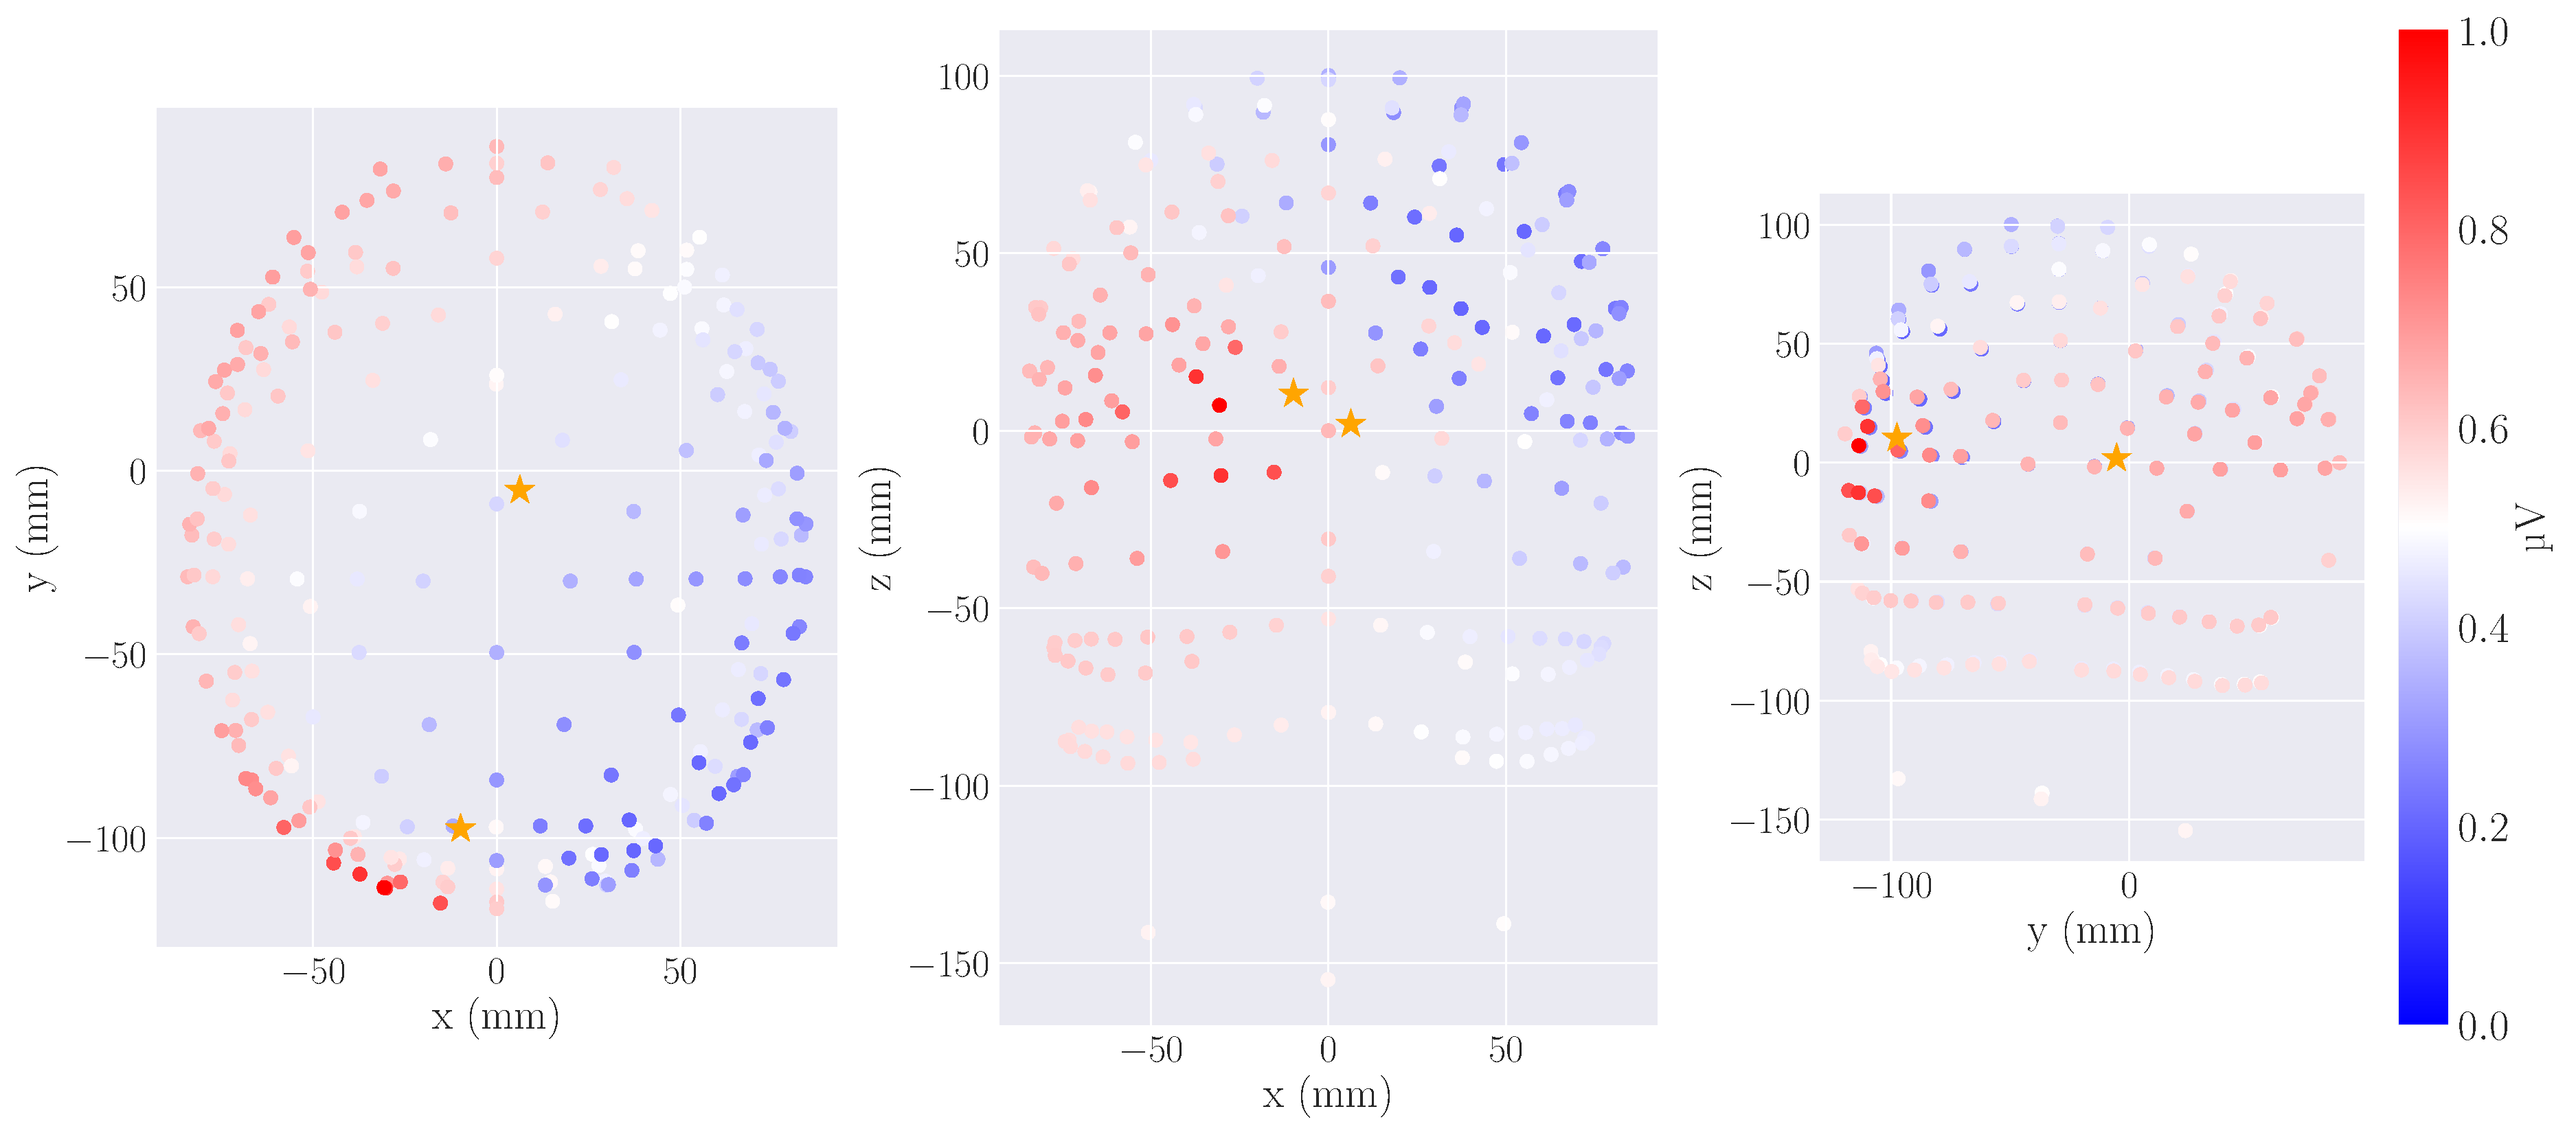
\includegraphics[width=\linewidth]{figures/dipoles_w_amplitudes_eeg_field_2_3.pdf}
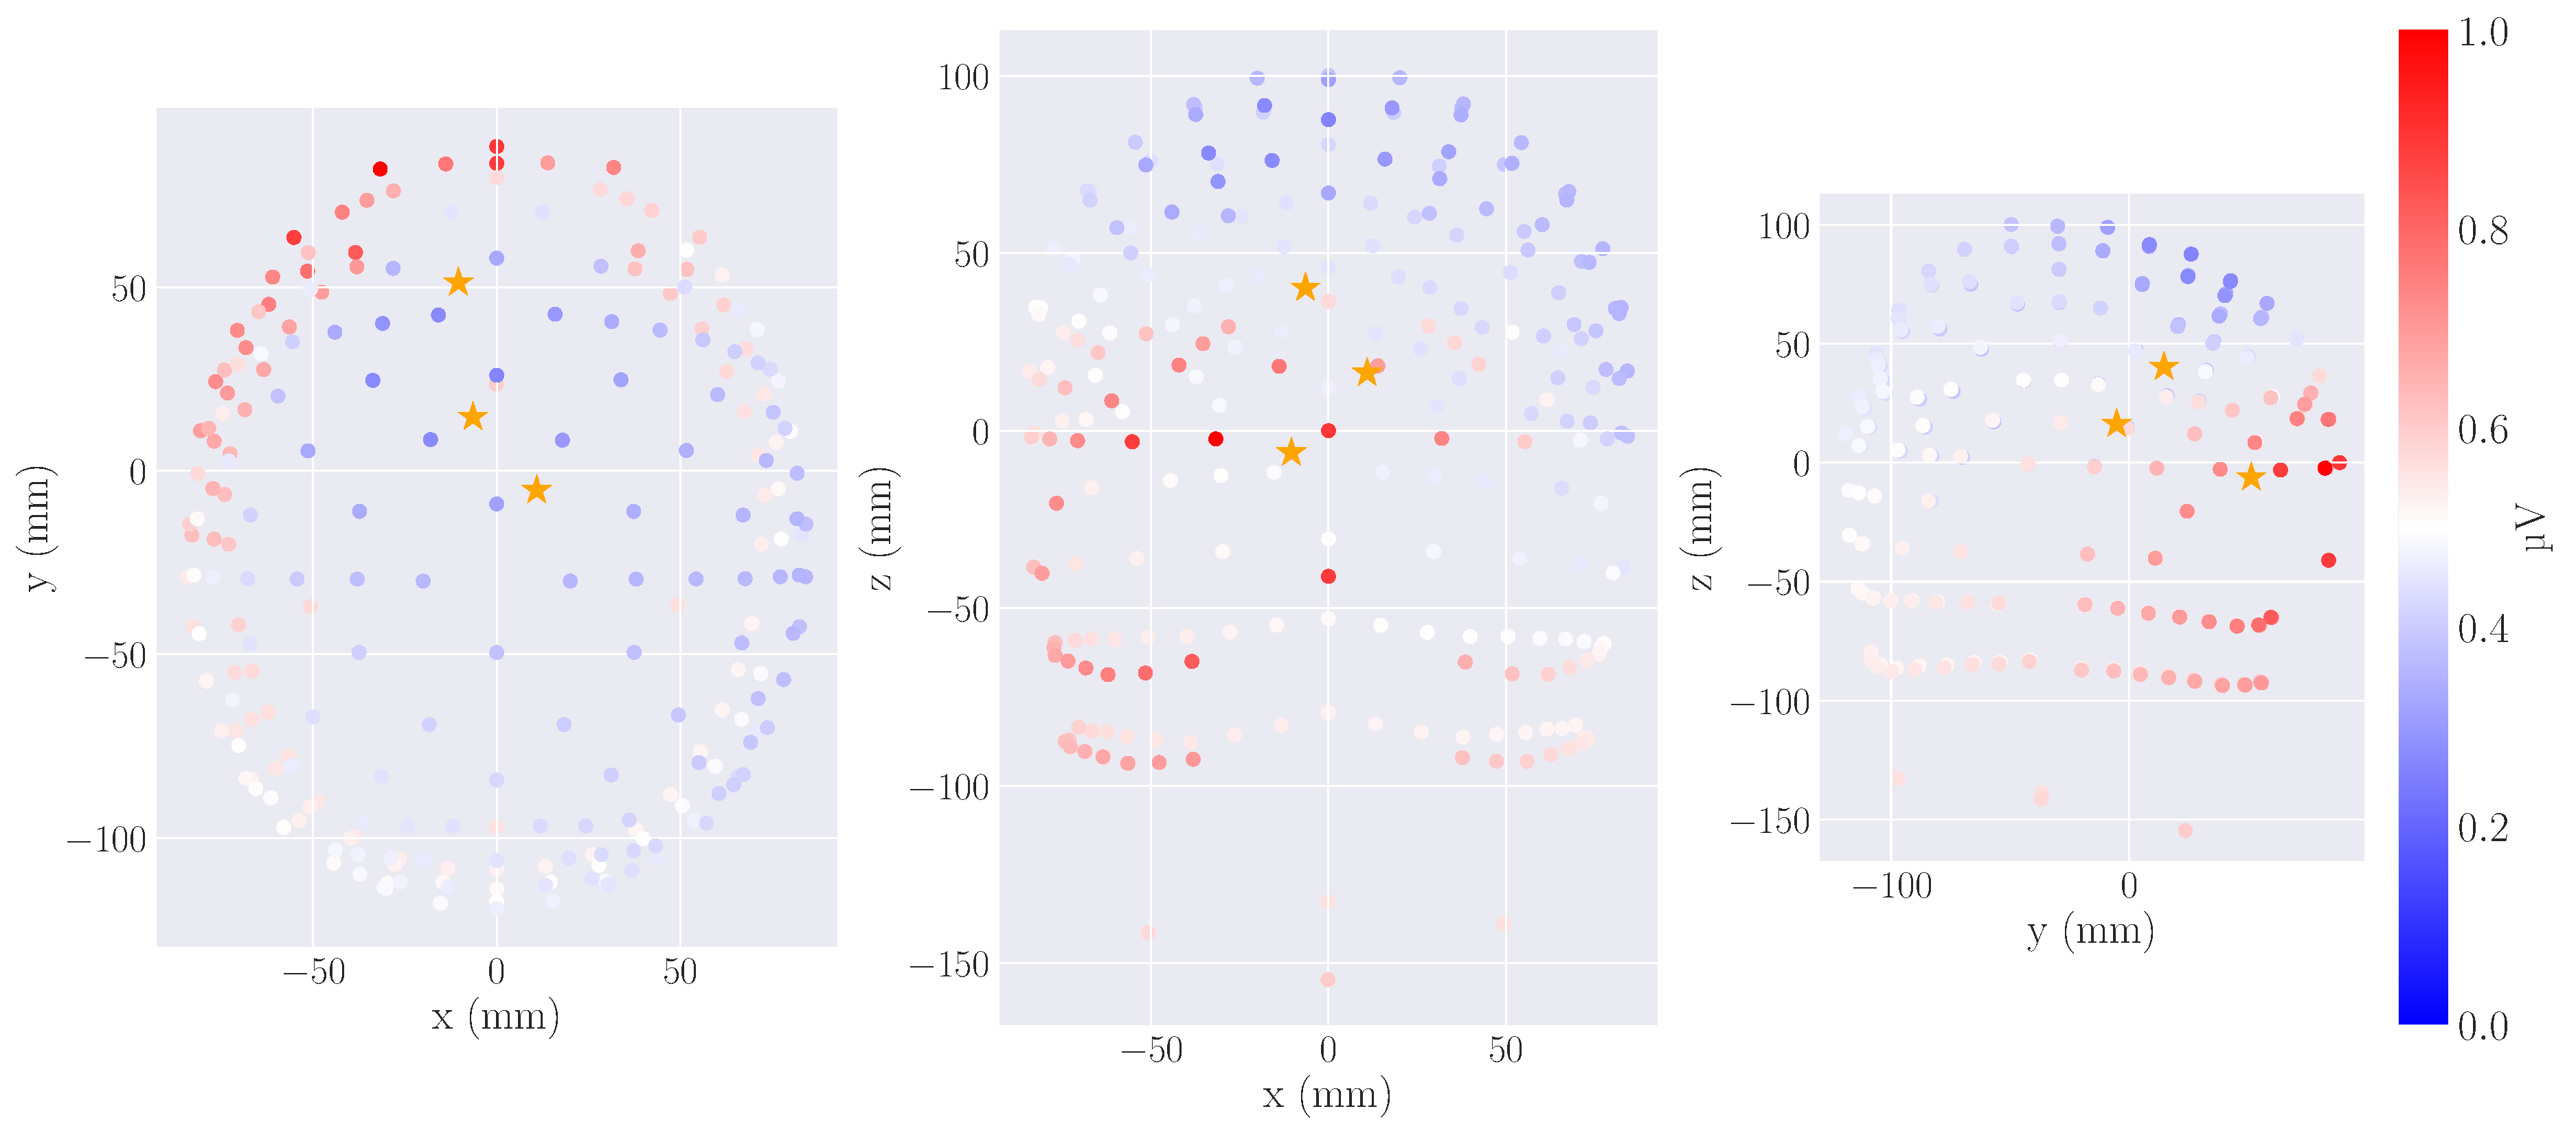
\includegraphics[width=\linewidth]{figures/dipoles_w_amplitudes_eeg_field_3_1.pdf}
\caption{EEG for two samples containing two and three current dipole sources, respectively, at random positions within the cerebral cortex. The EEG measures are seen from both sides (x-z plane and y-z plane) and from above the skull (x-y plane). EEG electrode locations are presented as filled circles, where the color of the fill represents the amplitude of the measured signal for the given electrode. The positions of the current dipole moments are marked with yellow stars.}
\label{fig:multiple_dipoles_data}
\end{figure}

The total number of target values for this problem has increased to 8, encompassing the x, y, and z-coordinates for the location, as well as the amplitude, of each dipole. Since we constrained each dipole within a sample to have the same amplitude, it is not necessary to have separate output values for the amplitudes of each dipole. Nevertheless, we modified the architecture of the network, considering the possibility of outputting amplitude target values with varying values for each dipole. Apart from this adjustment, the network still comprises 231 input nodes, and the target values have been normalized to range from 0 to 1. The logic and choice of activation functions, as well as hyperparameters, remain consistent with those used in previous problems. Figure \ref{fig:NN_multiple_dipoles_architecture} illustrates the updated network architecture.


\begin{figure}[!htb]
\centering
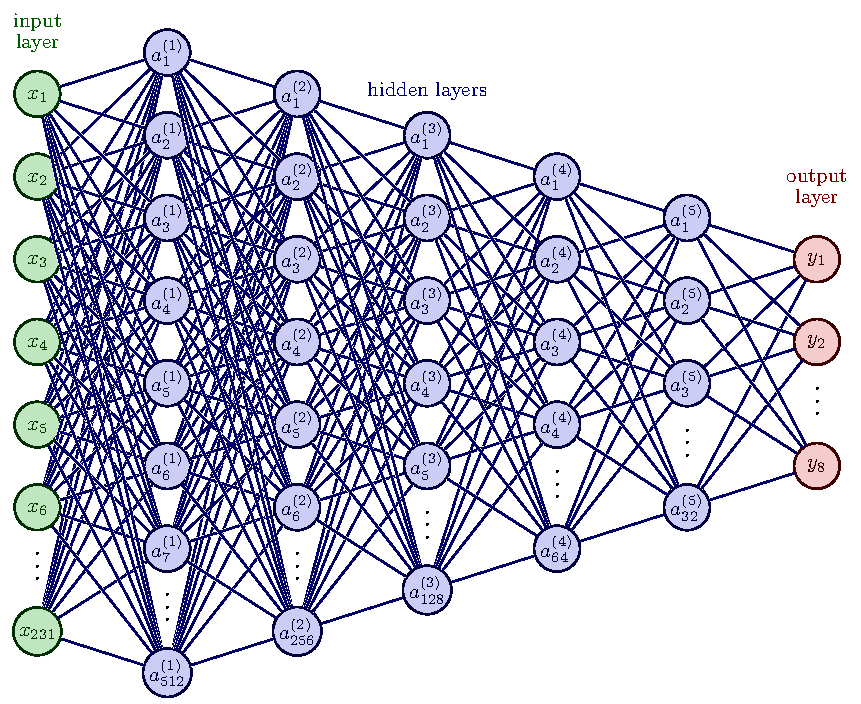
\includegraphics[width=\linewidth]{figures/NN_multiple_dipoles_architecture.pdf}
\caption{Architecture of the multiple dipoles network.}
\label{fig:NN_multiple_dipoles_architecture}
\end{figure}



\begin{figure}[!htb]
    \centering
    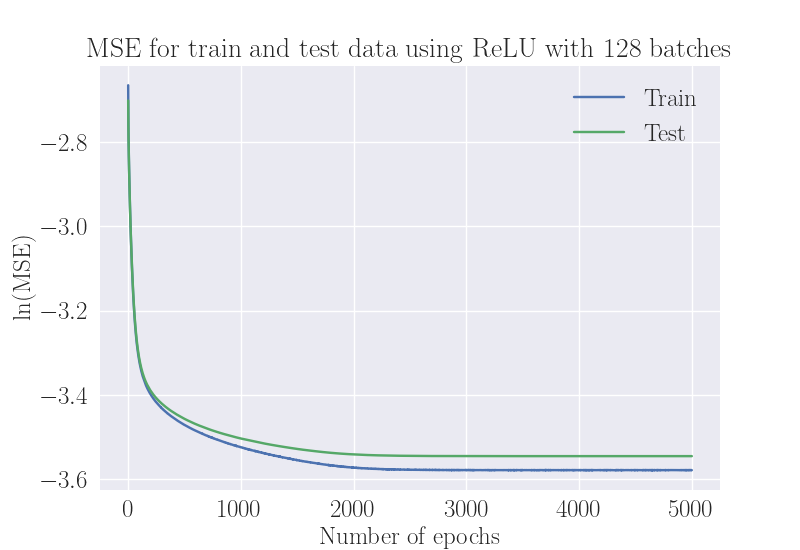
\includegraphics[width=\linewidth]{figures/MSE_26june_two_dipoles_w_amplitude_5000_SGD_lr0.001_wd0.1_mom0.35_bs128_10noise_ReLU_128_5000_N_dipoles_2.png}
    \caption{The validation accuracy for the simple Feed Forward Neural Network, predicting two current dipole sources.}
    \label{fig:dipole_area_result}
\end{figure}

\end{document}
